\section{Comparison With Other Deep Learning Frameworks}\label{sec:comp}

Next to TensorFlow, there exist a number of other open source deep learning
software libraries, the most popular being Theano, Torch and Caffe. In this
section, we review two sources of quantitative comparisons between TensorFlow
and other deep learning libraries, providing a summary of the most important
results of each work.

The first source in our collection is the \emph{convnet-benchmarks} repository
on GitHub by Soumith Chintala \cite{convnet-bench}, a research engineer at
Facebook. The commit we reference\footnote{Commit hash:
  84b5bb1785106e89691bc0625674b566a6c02147} is dated April 25, 2016. Chintala
provides an extensive set of benchmarks for a variety of convolutional network
models. Inter alia, Chintala gives the forward and backward-propagation time of
TensorFlow, Torch and Caffe --- but not Theano --- for the AlexNet CNN model
\cite{alexnet}. In these benchmarks, TensorFlow performs second-best in both
measures behind Torch, with Caffe lagging relatively far behind. We reproduce
the relevant results in Table \ref{tab:convnet}.

\begin{table}
  \centering
  \begin{tabular}{ccc}
    \textbf{Library} & \textbf{Forward (ms)} & \textbf{Backward (ms)}
    \\ \toprule
    TensorFlow & 26  & 55
    \\
    Torch & \textbf{25} & \textbf{46}
    \\
    Caffe & 121 & 203
    \\ \bottomrule
  \end{tabular}
  \caption{The result of Soumith Chintala's benchmarks for TensorFlow, Torch and
    Caffe (not Theano) on an AlexNet ConvNet model \cite{alexnet,
      convnet-bench}.}
  \label{tab:convnet}
\end{table}

Further benchmarks were published by the Theano development team in
\cite{theano} on May 9, 2016. We focus on their results for an LSTM network
operating on the Penn Treebank dataset \cite{penntreebank}. Their comparisons
measure words processed per second for a small model consisting of a single
200-unit hidden layer, and a large model with two 650-unit hidden
layers. Moreover, they used cuDNN v4 for all libraries included in their
benchmarks, which are TensorFlow, Torch and Theano. Results for Caffe are not
given. In their benchmarks, TensorFlow performs best among all three for the
small model, followed by Theano and then Torch. For the large model, TensorFlow
is placed second behind Theano, while Torch remains in last place. Table
\ref{fig:theano-results} shows these results.

\begin{figure}
  \centering
  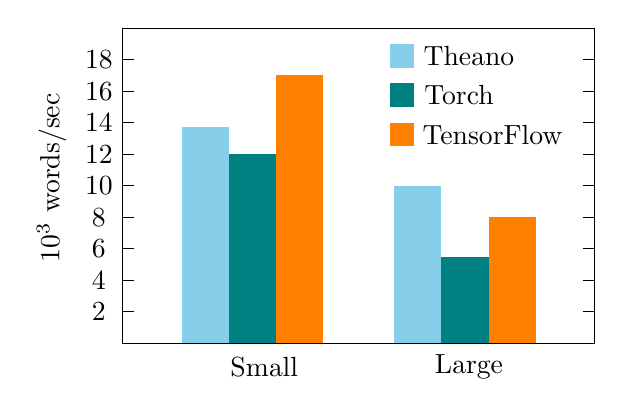
\begin{tikzpicture}
    % Frame
    \draw (0, 0) rectangle (6, 4);

    % Ticks + Scale
    \foreach \i in {2, 4, ..., 18} {
      % Left
      \draw (0, {\i / 5}) -- ++(+0.15, 0);
      % Right
      \draw (5.85, {\i / 5}) -- ++(+0.15, 0);
      % Labels
      \draw (-0.3, {\i / 5}) node {\i};
    }

    % Legend
    \draw (-0.9, 2.1) node [rotate=90] {$10^3$ words/sec};

    \fill [SkyBlue] (3.4, 3.5) rectangle ++(0.3, 0.3);
    \draw (4.4, 3.65) node {Theano};

    \fill [teal] (3.4, 3) rectangle ++(0.3, 0.3);
    \draw (4.275, 3.15) node {Torch};

    \fill [orange] (3.4, 2.5) rectangle ++(0.3, 0.3);
    \draw (4.7, 2.65) node {TensorFlow};


    %%% Small Model %%%

    % Theano
    \fill [SkyBlue] (0.75, 0) rectangle ++(0.6, 2.75);
    % Torch
    \fill [teal] (1.35, 0) rectangle ++(0.6, 2.4);
    % TensorFlow
    \fill [orange] (1.95, 0) rectangle ++(0.6, 3.4);

    % Label
    \draw (1.8, -0.3) node {Small};

    %%% Large Model %%%

    % Theano
    \fill [SkyBlue] (3.45, 0) rectangle ++(0.6, 2);
    % Torch
    \fill [teal] (4.05, 0) rectangle ++(0.6, 1.1);
    % TensorFlow
    \fill [orange] (4.65, 0) rectangle ++(0.6, 1.6);

    % Label
    \draw (4.4, -0.3) node {Large};

  \end{tikzpicture}
  \caption{The results of \cite{theano}, showing a comparison of TensorFlow,
    Theano and Torch on an LSTM model for the Penn Treebank dataset
    \cite{penntreebank}. On the left the authors tested a small model with a
    single hidden layer of 200 units; on the right they use two layers with 650
    units each. }
  \label{fig:theano-results}
\end{figure}

%%% Local Variables:
%%% mode: latex
%%% TeX-master: "../paper"
%%% End: